	% Set document type and scheme
	\documentclass[10pt]{beamer}
	\usetheme[progressbar=frametitle]{metropolis}

	% Load packages
	\usepackage{appendixnumberbeamer}
	\usepackage{booktabs}
	\usepackage[scale=2]{ccicons}
	\usepackage{pgfplots}
	\usepackage{xspace}
		\newcommand{\themename}{\textbf{\textsc{metropolis}}\xspace}
	\usepackage{stata}
	\usepackage{graphicx}

	\title{Stata Workshop} %% that will be typeset on the
	\subtitle{At MINAGRI} %% title page.
	\author{Roshni Khincha and Sakina Shibuya \\ DIME, World Bank}
	\date{August, 2018}

	\titlegraphic{%
		
\includegraphics[width=.2\textwidth]{DIME}\hfill % I think I should probably ask for a better image for this thing....
		
\includegraphics[width=.15\textwidth]{logo_minagri}\hfill
		
\includegraphics[width=.2\textwidth]{logo_eu}
		}

	\makeatletter
	\setbeamertemplate{title page}{
		\begin{minipage}[b][\paperheight]{\textwidth}
			\vfill%
			\ifx\inserttitle\@empty\else\usebeamertemplate*{title}\fi
			\ifx\insertsubtitle\@empty\else\usebeamertemplate*{subtitle}\fi
			\usebeamertemplate*{title separator}
			\ifx\beamer@shortauthor\@empty\else\usebeamertemplate*{author}\fi
			\ifx\insertdate\@empty\else\usebeamertemplate*{date}\fi
			\vfill
			\ifx\inserttitlegraphic\@empty\else\inserttitlegraphic\fi
			\vspace*{1cm}
		\end{minipage}
		}
	\makeatother

	\begin{document}
		
	\maketitle

	\section{Section 1}

		% 1.1 Why learn stata?
		\begin{frame}
		
			\frametitle{\textsc{Why learn stata?}}
			\begin{center}
				\textbf{Excel vs Stata} \\ \text{Can I use Excel?}
			\end{center}
		
		\end{frame}

		
		\begin{frame}
			\frametitle{\textsc{Why learn stata?}}
			\begin{center}
				\Large\textbf{The main reasons to use Stata}
			\end{center}
			\begin{itemize}
				\item In Excel you make changes directly to the data and save new versions of the data set
			
				\item In Stata you make changes to the instructions on how to get from the raw data to the final analysis and save new versions of the instructions
			
				\item Since Stata is a more statistics oriented software, processing the data to create analytical products can be a lot easier. 
			
			\end{itemize}
		\end{frame}



		\begin{frame}
			\frametitle{\textsc{The main reasons to use Stata}}
			\begin{center}
				\Large\textbf{The main reasons to use Stata}
			\end{center}
			\begin{itemize}
				\item Powerful tool with may capabilities:
				
				\begin{itemize}
					\item Descriptive statistics
					
					\item Inference statistics
					
					\item Complex data analysis
					
				\end{itemize}
				
				\item But it’s also good for beginner programmers:
				
				\begin{itemize}
					\item User friendly interface
					
					\item Relatively easy programming language that can be learned while you’re using the software
					
				\end{itemize}
			\end{itemize}
		\end{frame}	

		\begin{frame}
			\frametitle{\textsc{What's the fuss about do-files?}}
			\begin{center}
				\Large\textbf{What's the fuss about do-files?}
			\end{center}
			\begin{itemize}
				\item It’s through the do-file you communicate your work to other members in your team, both current and future
				\item Think of the do-files as instructions on how to get from raw data to final report
				\item For a simple task you can enter commands manually. But for more complex tasks you need to write a recipe, or a list of instructions
				
				\end{itemize}
			\end{frame}

		\begin{frame}

			\frametitle{\textsc{How to open up a data set in Stata?}}
			\begin{center}
				\textbf{How to open up a data set in Stata?} 
			\end{center}

		\end{frame}


		\begin{frame}
			\frametitle{\textsc{Three ways to tell Stata what to do}}
			\begin{center}
				\Large\textbf{Three ways to tell Stata what to do}
			\end{center}
			\begin{itemize}
				\item Drop-down menus
				
				\begin{itemize}
					\item An easy place to start but quickly becomes inefficient
					
				\end{itemize}
				
				\item Command window
				
			\begin{itemize}
				\item Faster than menus but require that you are familiar with the command
				
			\end{itemize}
				\item Do-file
				
			\begin{itemize}
				\item The only feasible way to run long instructions
				
				\item Use menus and command window to figure out what you need to write, then copy to a do file
				
			\end{itemize}
			\end{itemize}
		\end{frame}



		\begin{frame}
			\frametitle{\textsc{Open a dataset - menus}}
			\begin{center}
				\Large\textbf{Open a dataset - menus}
			\end{center}
			% \begin{figure}[H] 
			%	\centering
			%	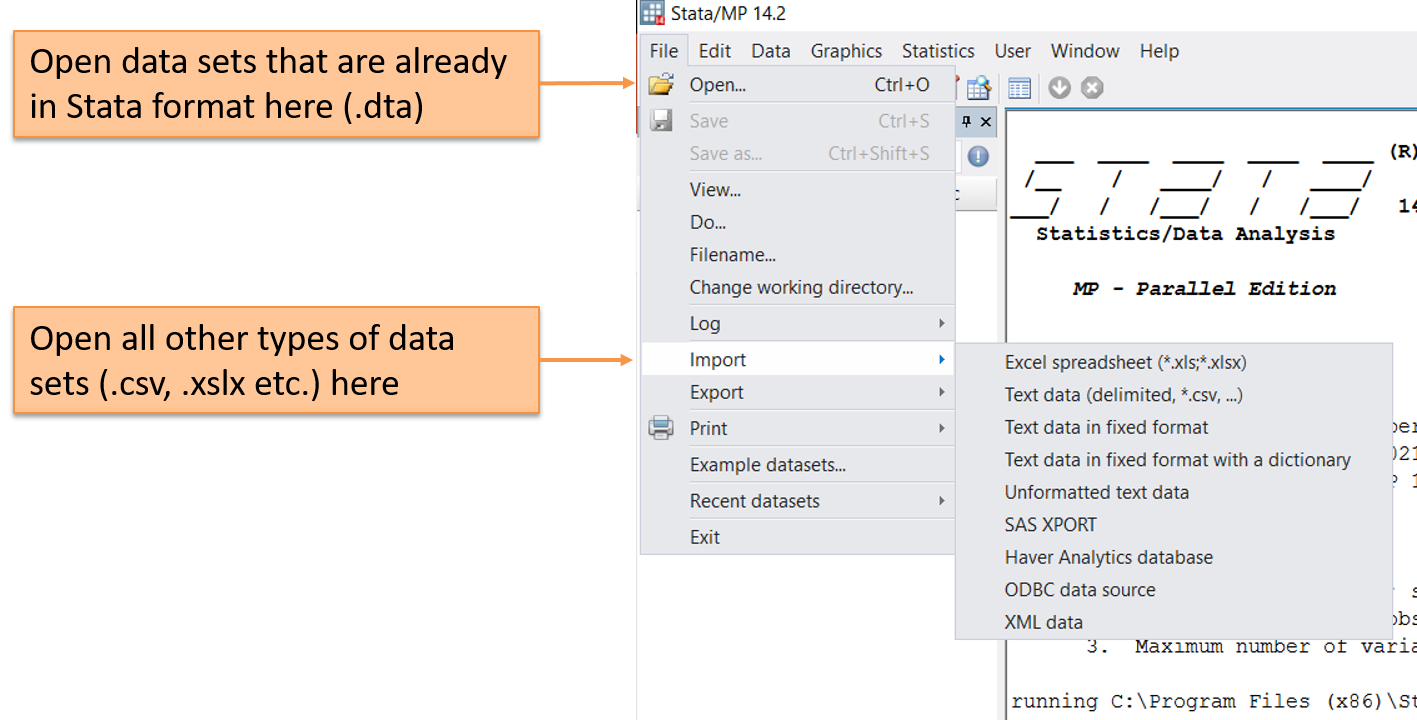
\includegraphics[width=0.9\linewidth]{../open_dataset_menu}
		%	\end{figure}
		\end{frame}

	\begin{frame}
		\frametitle{\textsc{Open a dataset – command windows}}
		\begin{center}
			\Large\textbf{Open a dataset – command window}
		\end{center}
		% \begin{figure}[H] 
		%	\centering
		%	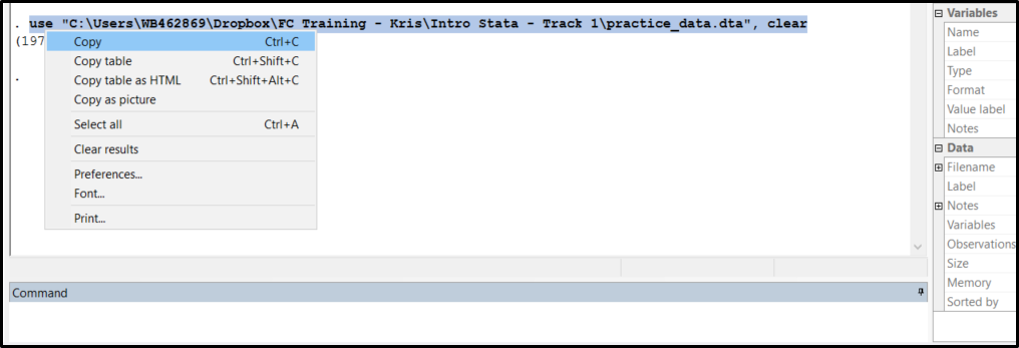
\includegraphics[width=0.9\linewidth]{../open_dataset_command}
		%	\end{figure}
		\begin{itemize}
			\item When you use the menus, Stata produces the code for that action (except for Data Browse)
			\begin{itemize}
				\item Highlight, right-click and copy the code
				\item Paste the code in the command window
				\item Hit enter
			\end{itemize}
		\end{itemize}
	\end{frame}


	\begin{frame}
		\frametitle{\textsc{Task 1}}
		\begin{center}
			\Large\textbf{Task 1}
		\end{center}
		\begin{enumerate}
			\item Open Stata and then open the EICV household data set \textbf{cs\_s0\_s5\_household.dta} using the menu: File $\rightarrow$ Open. Navigate to where you saved the material for this lab. Select the data set and click \textit{Open}
			\item Browse to check that you have data: Data  $\rightarrow$ Data Editor  $\rightarrow$ Data Editor Browse 
			\item Describe to get additional information on the data: Data  $\rightarrow$ Describe data $\rightarrow$ Describe data in memory or in a file.
			\begin{itemize}
				\item A new window will open
				\item Select In memory and press OK
			\end{itemize}
		\end{enumerate}
	\end{frame}

	\begin{frame}
		\frametitle{\textsc{Task 1}}
		\begin{center}
			\Large\textbf{Task 1}
		\end{center}
		\begin{itemize}
			\item You can see that one the second command printed information on your screen.
			\begin{itemize}
				\item The first part is the command used
				\item The second part are the results
			\end{itemize}
		\end{itemize}

		% \begin{figure}[H] 
			%	\centering
			%	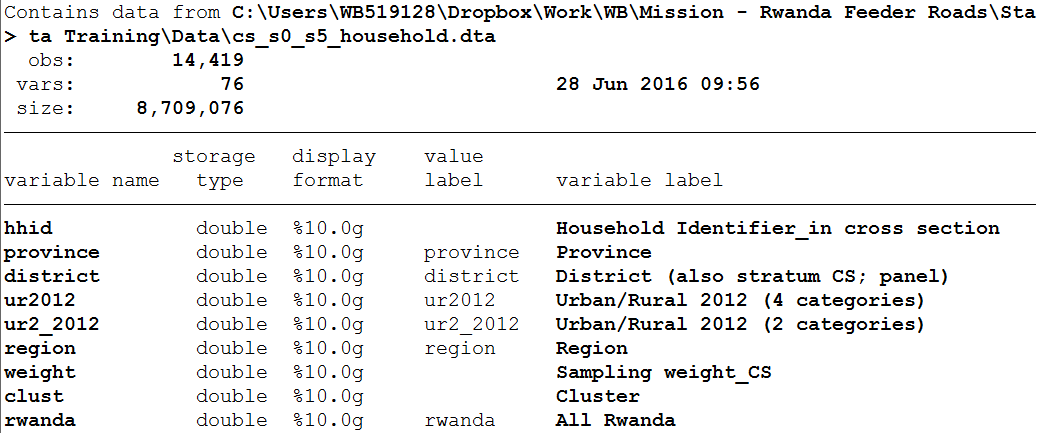
\includegraphics[width=0.9\linewidth]{../task1}
		%	\end{figure}
	\end{frame}



	\begin{frame}
		\frametitle{\textsc{Task 1}}
		\begin{center}
			\Large\textbf{Task 1}
		\end{center}
		\begin{itemize}
			\item You can perform both tasks by typing the in your command prompt. This will yield the same results
			
			\item Type \textit{browse} in the command window and press enter
			
			\item Type \textit{describe} and press enter
			
		\end{itemize}
	\end{frame}




	\begin{frame}
		\frametitle{\textsc{An introduction to Stata:Stata interface}}
		\begin{center}
			\textbf{An introduction to Stata} \\
			Stata interface
		\end{center}
	\end{frame}

	\begin{frame}
\frametitle{\textsc{}}
\begin{center}
	\Large\textbf{}
\end{center}
\begin{itemize}
	\item
\end{itemize}
\end{frame}


	\begin{frame}
\frametitle{\textsc{}}
\begin{center}
	\Large\textbf{}
\end{center}
\begin{itemize}
	\item
\end{itemize}
\end{frame}

	\begin{frame}
\frametitle{\textsc{}}
\begin{center}
	\Large\textbf{}
\end{center}
\begin{itemize}
	\item
\end{itemize}
\end{frame}
		
\section{Section 2}

	\begin{frame}
		\frametitle{\textsc{Edit data in Stata}}
		\begin{center}
			\textbf{How can we delete irrelevant variables?}
		\end{center}
	\end{frame}

	\begin{frame}[fragile]
		\frametitle{\textsc{Edit data in Stata}}
		\begin{center}
		\Large\textbf{Delete variables}
		\end{center}
		\begin{itemize}
		\item blah blah
		\end{itemize}
		\begin{stlog}tabulate s5bq3a
summarize s5bq3a 
codebook s5bq3a
\end{stlog}

\begin{stlog}tabulate s5bq3a
summarize s5bq3a 
codebook s5bq3a
\end{stlog}
	\end{frame}


	\section{Section 3}

	\end{document}
